\documentclass{standalone}
\usepackage{tikz}

\begin{document}
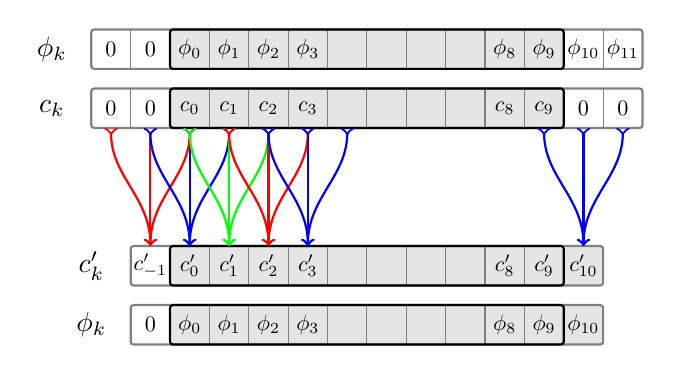
\begin{tikzpicture}
  \coordinate (com2) at (-0.75, 2.0);
  \coordinate (com1) at (-0.25, 2.0);
  \coordinate (co0) at (0.25, 2.0);
  \coordinate (co1) at (0.75, 2.0);
  \coordinate (co2) at (1.25, 2.0);
  \coordinate (co3) at (1.75, 2.0);
  \coordinate (co4) at (2.25, 2.0);
  \coordinate (co5) at (2.75, 2.0);
  \coordinate (co6) at (3.25, 2.0);
  \coordinate (co9) at (4.75, 2.0);
  \coordinate (co10) at (5.25, 2.0);
  \coordinate (co11) at (5.75, 2.0);

  \coordinate (cpm1) at (-0.25, 0.5);
  \coordinate (cp0) at (0.25, 0.5);
  \coordinate (cp1) at (0.75, 0.5);
  \coordinate (cp2) at (1.25, 0.5);
  \coordinate (cp3) at (1.75, 0.5);
  \coordinate (cp4) at (2.25, 0.5);
  \coordinate (cp5) at (2.75, 0.5);
  \coordinate (cp6) at (3.25, 0.5);
  \coordinate (cp8) at (4.25, 0.5);
  \coordinate (cp9) at (4.75, 0.5);
  \coordinate (cp10) at (5.25, 0.5);

  % upper
  \fill[gray!20, rounded corners=1] (0.0,2.75) rectangle (5.0,3.25);
  \foreach \i in {-1.0,-0.5,...,6.0} {
    \draw[gray] (\i,2.75) -- (\i,3.25);
  }
  \draw[gray, thick, rounded corners=1] (-1.0,2.75) rectangle (6.0,3.25);
  \draw[black, thick, rounded corners=1] (0.0,2.75) rectangle (5.0,3.25);

  \fill[gray!20, rounded corners=1] (0.0,2.0) rectangle (5.0,2.5);
  \foreach \i in {-1.0,-0.5,...,6.0} {
    \draw[gray] (\i,2.0) -- (\i,2.5);
  }
  \draw[gray, thick, rounded corners=1] (-1.0,2.0) rectangle (6.0,2.5);
  \draw[black, thick, rounded corners=1] (0.0,2.0) rectangle (5.0,2.5);

  % lower
  \fill[gray!20, rounded corners=1] (0.0,-0.75) rectangle (5.5,-0.25);
  \foreach \i in {0.0,0.5,...,5.0} {
    \draw[gray] (\i,-0.75) -- (\i,-0.25);
  }
  \draw[gray, thick, rounded corners=1] (-0.5,-0.75) rectangle (5.5,-0.25);
  \draw[black, thick, rounded corners=1] (0.0,-0.75) rectangle (5.0,-0.25);

  \fill[gray!20, rounded corners=1] (0.0,0.0) rectangle (5.5,0.5);
  \foreach \i in {0.0,0.5,...,5.0} {
    \draw[gray] (\i,0.0) -- (\i,0.5);
  }
  \draw[gray, thick, rounded corners=1] (-0.5,0.0) rectangle (5.5,0.5);
  \draw[black, thick, rounded corners=1] (0.0,0.0) rectangle (5.0,0.5);

  \draw[>->, thick, color=red] (com2) to[out=270,in=90] (cpm1);
  \draw[>->, thick, color=red] (com1) to[out=270,in=90] (cpm1);
  \draw[>->, thick, color=red] (co0) to[out=270,in=90] (cpm1);

  \draw[>->, thick, color=blue] (com1) to[out=270,in=90] (cp0);
  \draw[>->, thick, color=blue] (co0) to[out=270,in=90] (cp0);
  \draw[>->, thick, color=blue] (co1) to[out=270,in=90] (cp0);

  \draw[>->, thick, color=green] (co0) to[out=270,in=90] (cp1);
  \draw[>->, thick, color=green] (co1) to[out=270,in=90] (cp1);
  \draw[>->, thick, color=green] (co2) to[out=270,in=90] (cp1);

  \draw[>->, thick, color=red] (co1) to[out=270,in=90] (cp2);
  \draw[>->, thick, color=red] (co2) to[out=270,in=90] (cp2);
  \draw[>->, thick, color=red] (co3) to[out=270,in=90] (cp2);

  \draw[>->, thick, color=blue] (co2) to[out=270,in=90] (cp3);
  \draw[>->, thick, color=blue] (co3) to[out=270,in=90] (cp3);
  \draw[>->, thick, color=blue] (co4) to[out=270,in=90] (cp3);

  \draw[>->, thick, color=blue] (co9) to[out=270,in=90] (cp10);
  \draw[>->, thick, color=blue] (co10) to[out=270,in=90] (cp10);
  \draw[>->, thick, color=blue] (co11) to[out=270,in=90] (cp10);

  \node[scale=0.8] at (-0.75,2.25) [black] {$0$};
  \node[scale=0.8] at (-0.25,2.25) [black] {$0$};
  \node[scale=0.8] at (0.25,2.25) [black] {$c_0$};
  \node[scale=0.8] at (0.75,2.25) [black] {$c_1$};
  \node[scale=0.8] at (1.25,2.25) [black] {$c_2$};
  \node[scale=0.8] at (1.75,2.25) [black] {$c_3$};
  \node[scale=0.8] at (4.25,2.25) [black] {$c_8$};
  \node[scale=0.8] at (4.75,2.25) [black] {$c_9$};
  \node[scale=0.8] at (5.25,2.25) [black] {$0$};
  \node[scale=0.8] at (5.75,2.25) [black] {$0$};

  \node[scale=0.8] at (-0.25,0.25) [black] {$c^\prime_{-1}$};
  \node[scale=0.8] at (0.25,0.25) [black] {$c^\prime_0$};
  \node[scale=0.8] at (0.75,0.25) [black] {$c^\prime_1$};
  \node[scale=0.8] at (1.25,0.25) [black] {$c^\prime_2$};
  \node[scale=0.8] at (1.75,0.25) [black] {$c^\prime_3$};
  \node[scale=0.8] at (4.25,0.25) [black] {$c^\prime_8$};
  \node[scale=0.8] at (4.75,0.25) [black] {$c^\prime_9$};
  \node[scale=0.8] at (5.25,0.25) [black] {$c^\prime_{10}$};

  \node[scale=0.8] at (-0.75,3.0) [black] {$0$};
  \node[scale=0.8] at (-0.25,3.0) [black] {$0$};
  \node[scale=0.8] at (0.25,3.0) [black] {$\phi_0$};
  \node[scale=0.8] at (0.75,3.0) [black] {$\phi_1$};
  \node[scale=0.8] at (1.25,3.0) [black] {$\phi_2$};
  \node[scale=0.8] at (1.75,3.0) [black] {$\phi_3$};
  \node[scale=0.8] at (4.25,3.0) [black] {$\phi_8$};
  \node[scale=0.8] at (4.75,3.0) [black] {$\phi_9$};
  \node[scale=0.8] at (5.25,3.0) [black] {$\phi_{10}$};
  \node[scale=0.8] at (5.75,3.0) [black] {$\phi_{11}$};

  \node[scale=0.8] at (-0.25,-0.5) [black] {$0$};
  \node[scale=0.8] at (0.25,-0.5) [black] {$\phi_0$};
  \node[scale=0.8] at (0.75,-0.5) [black] {$\phi_1$};
  \node[scale=0.8] at (1.25,-0.5) [black] {$\phi_2$};
  \node[scale=0.8] at (1.75,-0.5) [black] {$\phi_3$};
  \node[scale=0.8] at (4.25,-0.5) [black] {$\phi_8$};
  \node[scale=0.8] at (4.75,-0.5) [black] {$\phi_9$};
  \node[scale=0.8] at (5.25,-0.5) [black] {$\phi_{10}$};

  \node at (-1.5,3.0) [black] {$\phi_{k}$};
  \node at (-1.0,-0.5) [black] {$\phi_{k}$};
  \node at (-1.5,2.25) [black] {$c_{k}$};
  \node at (-1.0,0.25) [black] {$c^\prime_{k}$};
\end{tikzpicture}
\end{document}
